
%(BEGIN_QUESTION)
% Copyright 2015, Tony R. Kuphaldt, released under the Creative Commons Attribution License (v 1.0)
% This means you may do almost anything with this work of mine, so long as you give me proper credit

Identify the effects of the following faults in this protective relay DC trip circuit:

$$\includegraphics[width=15.5cm]{i03098x01.eps}$$

\begin{itemize}
\item{} Upper resistor failing open
\vskip 10pt
\item{} Upper capacitor failing shorted
\vskip 10pt
\item{} Loose connection on left side of terminal 12
\vskip 10pt
\item{} Broken wire between terminals D and 10
\vskip 10pt
\item{} Broken wire between terminals E and 11
\vskip 10pt
\item{} Ground fault at terminal 7
\vskip 10pt
\item{} Simultaneous ground faults at terminals 9 and 6
\end{itemize}

\vskip 20pt \vbox{\hrule \hbox{\strut \vrule{} {\bf Suggestions for Socratic discussion} \vrule} \hrule}

\begin{itemize}
\item{} What is the point of having both 5 amp and 10 amp fuses in this circuit?
\item{} What should a voltmeter register between terminal 3 and ground?  Between terminal 4 and ground?  If we permanently installed two voltmeters to register these voltages, could their indications help us pinpoint certain faults before they become serious?
\item{} Can we tell what ANSI/IEEE function this protective relay implements?  Why or why not?
\end{itemize}

\underbar{file i03098}
%(END_QUESTION)





%(BEGIN_ANSWER)

\noindent
{\bf Partial answer:}

\begin{itemize}
\item{} Upper capacitor failing shorted: {\it Negative DC bus line goes to ground potential ; Positive DC bus line rises to +130 VDC above ground potential.} 
\vskip 5pt
\item{} Loose connection on left side of terminal 12: {\it Indicator lamp refuses to energize when relay contact OUT2 asserts ; AC power circuit breaker refuses to trip when relay contact OUT1 asserts.}
\vskip 5pt
\item{} Broken wire between terminals E and 11: {\it Indicator lamp refuses to energize when relay contact OUT2 asserts.}
\end{itemize}

%(END_ANSWER)





%(BEGIN_NOTES)

\begin{itemize}
\item{} Upper resistor failing open: {\it Negative DC bus line goes to ground potential ; Positive DC bus line rises to +130 VDC above ground potential ; no effect on system operation.}
\vskip 5pt
\item{} Upper capacitor failing shorted: {\it Negative DC bus line goes to ground potential ; Positive DC bus line rises to +130 VDC above ground potential ; no effect on system operation.} 
\vskip 5pt
\item{} Loose connection on left side of terminal 12: {\it Indicator lamp refuses to energize when relay contact OUT2 asserts ; AC power circuit breaker refuses to trip when relay contact OUT1 asserts.}
\vskip 5pt
\item{} Broken wire between terminals D and 10: {\it Relay will ``think'' the circuit breaker is tripped (open) even when it isn't.}
\vskip 5pt
\item{} Broken wire between terminals E and 11: {\it Indicator lamp refuses to energize when relay contact OUT2 asserts.}
\vskip 5pt
\item{} Ground fault at terminal 7: {\it Positive DC bus line goes to ground potential ; Negative DC bus line sinks to $-130$ VDC below ground potential ; no effect on system operation.}
\vskip 5pt
\item{} Simultaneous ground faults at terminals 9 and 6: {\it One or both of the 5 amp fuses will blow.}
\end{itemize}

%INDEX% Protective relay: troubleshooting

%(END_NOTES)


